\documentclass[12pt,letterpaper]{article}

% ===================== PAQUETES =====================
\usepackage[spanish,es-tabla]{babel}
\usepackage[utf8]{inputenc}
\usepackage[T1]{fontenc}
\usepackage{geometry}
\usepackage{graphicx}
\usepackage{float}
\usepackage{booktabs}
\usepackage{array}
\usepackage{longtable}
\usepackage{tabularx}
\usepackage{enumitem}
\usepackage{hyperref}
\usepackage{xcolor}
\usepackage{titlesec}
\usepackage{fancyhdr}
\usepackage{pgfgantt}
\usepackage{tikz}
\usepackage{pgfplots}

\pgfplotsset{compat=1.18}
\geometry{margin=2.5cm}
\hypersetup{colorlinks=true, linkcolor=black, urlcolor=blue, citecolor=black}

% ===================== DATOS =====================
\newcommand{\nombreProyecto}{VitalCode: Entorno Virtual de Primeros Auxilios Psicológicos}
\newcommand{\nombreCurso}{Ingeniería y Desarrollo Sustentable/Sostenible}
\newcommand{\docentes}{Pía Del Canto C. -- Aracelly Aravena F.}
\newcommand{\ayudantes}{Anyel Cortés -- Jorge Herrera}
\newcommand{\grupo}{VitalCode}
\newcommand{\integrantes}{Elliot Bravo, Catalina Rojas, Matías Collao, Benjamín Cortés}
\newcommand{\fecha}{Junio 2026}

\pagestyle{fancy}
\fancyhf{}
\lhead{\grupo}
\rhead{Informe Final IDS}
\cfoot{\thepage}

\titleformat{\section}{\large\bfseries}{\thesection.}{0.5em}{}
\titleformat{\subsection}{\normalsize\bfseries}{\thesubsection.}{0.5em}{}

\begin{document}

% ===================== PORTADA =====================
\begin{titlepage}
\centering
\vspace*{1cm}
{\Large \textbf{\nombreCurso}}\\[0.4cm]
{\large Informe Final de Proyecto}\\[1.5cm]
{\Huge \textbf{\nombreProyecto}}\\[1cm]
{\Large \textbf{Grupo:} \grupo}\\[0.4cm]
{\large \textbf{Integrantes:} \integrantes}\\[0.4cm]
{\large \textbf{Docentes:} \docentes}\\[0.2cm]
{\large \textbf{Ayudantes:} \ayudantes}\\[1cm]
{\large \textbf{ODS principal:} ODS 3 -- Salud y Bienestar}\\[2cm]
{\large \fecha}
\vfill
\end{titlepage}

\tableofcontents
\newpage

% ===================== RESUMEN =====================
\section*{Resumen}
\addcontentsline{toc}{section}{Resumen}
El presente informe final desarrolla la propuesta \textit{VitalCode}, una aplicación orientada a democratizar el acceso a la salud mental de adolescentes mediante recursos digitales de primeros auxilios psicológicos (PAP). El proyecto se vincula directamente con el ODS 3 (Salud y Bienestar) al reducir barreras de acceso y estigma. Desde el enfoque de la ingeniería, se plantea como una solución de "Producción Limpia", utilizando estrategias de Green Computing, desmaterialización y eficiencia energética para garantizar la sostenibilidad ambiental, económica y social del servicio.

\textbf{Palabras clave:} salud mental, ODS 3, aplicación, primeros auxilios psicológicos, producción limpia, sostenibilidad, QHSEC.

\newpage

% ===================== 1 CONTEXTO =====================
\section{Contexto del proyecto}

\subsection{Descripción general de la empresa}
\textbf{VitalCode SpA} es una empresa del sector tecnológico (desarrollo de software) orientada al diseño de soluciones digitales para el bienestar psicológico adolescente. Su producto principal es una aplicación \textit{lightweight} (ligera) que permite a los usuarios acceder de manera anónima a recursos de apoyo emocional y primeros auxilios psicológicos. Al ser una PYME digital, su modelo operativo tiene un impacto logístico nulo, optimizando los recursos mediante computación en la nube.

\subsection{Estructura organizacional}
Para cumplir con los lineamientos, la empresa considera la siguiente estructura, integrando áreas técnicas y científicas:

\begin{table}[H]
\centering
\caption{Estructura organizacional de VitalCode}
\begin{tabularx}{\textwidth}{p{4.5cm} X}
\toprule
\textbf{Cargo / Área} & \textbf{Función principal} \\
\midrule
Gerente General & Dirección estratégica, planeación y alianzas institucionales. \\
Director Tecnológico (CTO) & Liderar el desarrollo de la app, arquitectura de software y nube. \\
Psicólogo/a Clínico (Jefe) & Validar protocolos clínicos y contenidos de los PAP. \\
Especialista en Crisis & Asegurar la pertinencia del abordaje en situaciones de alto estrés. \\
Desarrolladores Móviles (2) & Programación y optimización de código bajo estándares \textit{Green IT}. \\
Analista de Ciberseguridad & Protección de datos sensibles y cumplimiento normativo (Ley 19.628). \\
\bottomrule
\end{tabularx}
\end{table}

\subsection{Misión y visión}
\textbf{Misión:} Democratizar el acceso a herramientas de contención emocional mediante tecnología móvil segura, eficiente e inclusiva.

\textbf{Visión:} Ser la plataforma líder a nivel nacional en primeros auxilios psicológicos asíncronos, promoviendo el bienestar juvenil y reduciendo la carga sobre el sistema público de salud bajo un modelo de desarrollo tecnológico sostenible.

% ===================== 2 PROBLEMA =====================
\section{Descripción del problema y oportunidad}

La alta prevalencia de crisis de ansiedad y estrés en jóvenes chilenos constituye una problemática social severa. El acceso oportuno a la salud mental está severamente limitado por barreras económicas, estigma social y la saturación del sistema público.

\textbf{Oportunidad:} La altísima tasa de presencia de smartphones en la población joven permite entregar una herramienta de Primeros Auxilios Psicológicos (PAP) asíncrona, anónima y de bolsillo. Esta solución tiene un impacto directo en el \textbf{ODS 3 (Salud y Bienestar)} promoviendo la contención emocional inicial, y adicionalmente, democratiza el acceso a herramientas de salud, impactando positivamente en el \textbf{ODS 10 (Reducción de las Desigualdades)}.

% ===================== 3 ANALISIS ENTORNO =====================
\section{Análisis del entorno}

\subsection{Análisis Interno: FODA}
\begin{itemize}[leftmargin=*]
    \item \textbf{Fortalezas:} Bajos costos operativos por infraestructura digital; accesibilidad 24/7; anonimato garantizado.
    \item \textbf{Debilidades:} Dependencia estructural de profesionales externos para validación clínica; requerimiento de conexión a internet para uso completo.
    \item \textbf{Oportunidades:} Demanda creciente por concientización en salud mental juvenil; impulso gubernamental hacia la telemedicina.
    \item \textbf{Amenazas:} Alta competencia de apps internacionales (ej. Calm); regulación estricta en el manejo de datos médicos.
\end{itemize}

\subsection{Análisis Externo: PESTEL}
\begin{itemize}[leftmargin=*]
    \item \textbf{Político:} Políticas públicas orientadas a la modernización de los planes de salud mental y prevención del suicidio.
    \item \textbf{Económico:} La reducción del poder adquisitivo hace atractivas las soluciones tecnológicas de bajo costo o gratuitas.
    \item \textbf{Social:} Desestigmatización de la terapia en jóvenes y aumento del estrés crónico derivado de crisis sociales.
    \item \textbf{Tecnológico:} Expansión del 5G y masificación de smartphones en todos los estratos socioeconómicos.
    \item \textbf{Ecológico:} Aplicación de \textit{Green Computing} y uso de servidores alojados en centros de datos con energías renovables.
    \item \textbf{Legal:} Obligatoriedad de cumplir la Ley 19.628 de Protección a la Vida Privada.
\end{itemize}

\subsection{Análisis Externo: 5 Fuerzas de Porter}
\begin{enumerate}[leftmargin=*]
\item \textbf{Rivalidad de competidores (Media):} Existen gigantes globales de meditación, pero pocas enfocadas estrictamente en "Primeros Auxilios Psicológicos" locales.
\item \textbf{Nuevos entrantes (Media-Alta):} Barrera tecnológica baja, pero altísima barrera de entrada en "confianza y validación clínica".
\item \textbf{Negociación de proveedores (Baja):} Existe una amplia oferta de servicios de \textit{Cloud Hosting} (AWS, Azure). Además, al utilizar frameworks de código abierto como React Native apoyados por los servicios de compilación de Expo (EAS), se evita la dependencia o monopolio de un solo proveedor tecnológico costoso.
\item \textbf{Negociación de clientes (Alta):} Costo de cambio cero; los usuarios pueden desinstalar la app sin pérdida financiera.
\item \textbf{Amenaza de sustitutos (Alta):} Líneas telefónicas del Estado ("Salud Responde") y evasión a través de redes sociales.
\end{enumerate}

% ===================== 4 PLANEACION =====================
\section{Planeación administrativa del proyecto}

\subsection{Identificación de recursos}
\begin{itemize}[leftmargin=*]
    \item \textbf{Recursos Físicos y Tecnológicos:} Laptops de alta eficiencia para los desarrolladores, smartphones para la ejecución de la maqueta en vivo mediante la aplicación \textit{Expo Go}, y el uso del framework React Native (Expo) para el desarrollo ágil.
    \item \textbf{Recursos Económicos:} Presupuesto inicial para cubrir servidores Cloud (Hosting), servicios de compilación en la nube (Expo Application Services - EAS), salarios del equipo núcleo y campañas de marketing digital.
    \item \textbf{Recursos Humanos:} Detallados en la estructura organizacional (Ingenieros, psicólogos clínicos, diseñador UX/UI).
\end{itemize}

\subsection{Presupuesto estimado}
Para la ejecución del proyecto, se ha definido una estructura de costos basada en un modelo operativo eficiente de software, priorizando los servicios en la nube bajo demanda y la validación profesional de contenidos.

\begin{table}[H]
\centering
\caption{Presupuesto estimado del proyecto VitalCode (CLP)}
\begin{tabularx}{\textwidth}{X r}
\toprule
\textbf{Ítem} & \textbf{Costo estimado (CLP)} \\
\midrule
Infraestructura Cloud (Firebase/EAS) & 120.000 \\
Honorarios Asesoría Clínica (Psicólogo) & 250.000 \\
Licencias de software y herramientas & 80.000 \\
Marketing y difusión digital & 100.000 \\
Imprevistos (10\%) & 55.000 \\
\midrule
\textbf{TOTAL ESTIMADO} & \textbf{605.000} \\
\bottomrule
\end{tabularx}
\end{table}

\subsection{Cronograma (Carta Gantt)}
Para la ejecución del proyecto VitalCode, se estructuró un cronograma de 13 periodos de trabajo, iniciando con la ideación a fines de marzo y culminando con la presentación del prototipo y entrega final a fines de junio.

\begin{figure}[H]
\centering
\resizebox{\textwidth}{!}{
\begin{ganttchart}[
hgrid,
vgrid,
x unit=0.8cm,
y unit chart=0.55cm,
title height=1,
bar height=0.6,
bar/.append style={fill=green!80, rounded corners=2pt}
]{1}{13}
% Títulos de los meses
\gantttitle{Marzo}{1} \gantttitle{Abril}{4} \gantttitle{Mayo}{4} \gantttitle{Junio}{4} \\
% Número de semanas / periodos
\gantttitlelist{1,...,13}{1} \\
% Tareas alineadas según la imagen
\ganttbar{1. Lluvia de ideas y planteamiento}{1}{2} \\
\ganttbar{2. Análisis del problema (ODS 3)}{2}{3} \\
\ganttbar{3. Formalización de la idea (VitalCode)}{4}{5} \\
\ganttbar{4. Encuestas de validación}{5}{6} \\
\ganttbar{5. Análisis estratégico (FODA, PESTEL, Porter)}{6}{8} \\
\ganttbar{6. Diseño de Interfaz UI/UX (Prototipo)}{7}{9} \\
\ganttbar{7. Integración, Sostenibilidad y QHSEC}{9}{10} \\
\ganttbar{8. Refinamiento de Maqueta}{9}{11} \\
\ganttbar{9. Redacción de informe final}{11}{12} \\
\ganttbar{10. Preparación de defensa y Entrega final}{13}{13}
\end{ganttchart}
}
\caption{Carta Gantt detallada del proyecto VitalCode.}
\end{figure}

% ===================== 5 PRODUCCION LIMPIA =====================
\section{Producción Limpia y Localización}

\subsection{Establecimiento y Localización}
VitalCode opera bajo un modelo de \textbf{teletrabajo híbrido}. La sede corporativa (oficina comercial y legal) se localiza en un espacio de \textit{Coworking} en la ciudad de Coquimbo, Chile. Esta decisión es estratégica: evita la construcción de infraestructura física propia, minimizando el impacto ambiental por urbanización y centralizando servicios (luz, agua, internet) compartidos con otras empresas.

\begin{figure}[H]
\centering
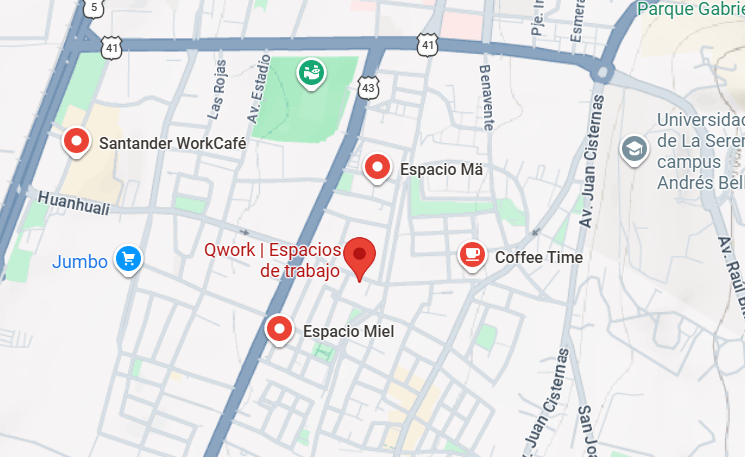
\includegraphics[width=0.8\textwidth]{image.png}
\caption{Mapa de localización referencial - Centro de Coworking, Coquimbo.}
\end{figure}

\subsection{Estrategias de Producción Limpia}
Al ser una aplicación digital, el enfoque de Producción Limpia se rige por la \textbf{Informática Verde (Green Computing)} y la \textbf{Desmaterialización}:
\begin{itemize}[leftmargin=*]
    \item \textbf{Eficiencia Cross-Platform (Arquitectura Expo):} Al utilizar React Native y Expo, la aplicación emplea un único código base que compila simultáneamente para Android e iOS. Esto reduce drásticamente las horas de cómputo necesarias y el consumo energético en servidores, al no tener que mantener ni compilar dos repositorios de código por separado.
    \item \textbf{Diseño Eficiente (Dark Mode):} La interfaz utiliza fondos oscuros por defecto, apagando píxeles en pantallas OLED. Esto minimiza el consumo de batería y prolonga la vida útil del smartphone, retrasando la generación de chatarra electrónica (\textit{e-waste}).
    \item \textbf{Desmaterialización Logística:} La distribución netamente digital a través de App Stores elimina el transporte físico, embalajes plásticos y las emisiones de Gases de Efecto Invernadero (GEI) de las cadenas de suministro.
    \item \textbf{Hosting Sustentable (Cloud Computing):} La base de datos y el backend operan bajo Firebase (Google Cloud), un proveedor que garantiza igualar el 100\% del consumo eléctrico de sus centros de datos con compras de energía renovable, mitigando la huella de la etapa operativa.
\end{itemize}

% ===================== 6 QHSEC Y CICLO DE VIDA =====================
\section{Gestión Integrada Q-HSEC y Ciclo de Vida}

\subsection{Sistema Integrado Q-HSEC}
La gestión de VitalCode se sustenta en principios normativos de calidad, ambiente y seguridad, aplicados al desarrollo de software:

\begin{table}[H]
\centering
\caption{Matriz de Gestión Integrada Q-HSEC}
\begin{tabularx}{\textwidth}{c X}
\toprule
\textbf{Dimensión} & \textbf{Plan de Gestión (Concordancia Normativa)} \\
\midrule
\textbf{Q (Calidad)} & \textit{Base ISO 9001:} Validación estricta de todos los ejercicios por profesionales de la salud para asegurar efectividad. \\
\textbf{H (Salud)} & Prevención de riesgos ergonómicos y síndrome de \textit{burnout} en los desarrolladores mediante pausas activas y desconexión digital. \\
\textbf{S (Seguridad)} & \textit{Base ISO 45001:} Protección de datos sensibles con encriptación de extremo a extremo en Firebase y uso de avatares para no exponer identidad real. \\
\textbf{E (Ambiente)} & \textit{Base ISO 14001:} Operación con impacto minimizado alojando el backend en Google Cloud (100\% energías renovables). \\
\textbf{C (Comunidad)} & Aporte directo al ODS 3, descongestionando la red pública y democratizando el acceso a contención emocional. \\
\bottomrule
\end{tabularx}
\end{table}

\subsection{Gestión de Huellas y Ciclo de Vida}
\begin{itemize}[leftmargin=*]
    \item \textbf{Huella de Carbono (Operación):} Es el punto crítico. Se mitiga mediante el alojamiento en servidores Cloud ecológicos. Utilizando \textit{Website Carbon Calculator}, se estima una huella de apenas 0.2g de $CO_2$ por sesión.
    \item \textbf{Huella Hídrica:} Virtualmente cero, dado que no existen procesos de manufactura física ni refrigeración industrial propia.
    \item \textbf{Ciclo de Uso (Dark Mode):} La interfaz oscura por defecto apaga píxeles en pantallas OLED, reduciendo el consumo de batería y prolongando la vida útil del smartphone del usuario.
    \item \textbf{Fin de Vida limpio:} La desinstalación de la aplicación no genera ningún tipo de residuo sólido ni chatarra electrónica (\textit{e-waste}).
\end{itemize}

% ===================== 7 LEGISLACION =====================
\section{Legislación Vigente}

\subsection{Orientada a la Sustentabilidad y Privacidad (Usuarios)}
\begin{itemize}[leftmargin=*]
    \item \textbf{Ley N° 19.300 (Bases Generales del Medio Ambiente):} Al ser un proyecto 100\% digital y operar mediante \textit{Coworking}, VitalCode no requiere someterse al SEIA, ya que sus operaciones no generan emisiones directas ni residuos sólidos.
    \item \textbf{Ley N° 19.628 (Protección de la Vida Privada):} Al tratar datos "sensibles" sobre el estado emocional, se cumple anonimizando perfiles y prohibiendo la comercialización de la base de datos.
    \item \textbf{Ley N° 20.584 (Derechos y Deberes de los Pacientes):} Se respetan sus principios entregando "Términos y Condiciones" claros, estipulando que la app es de primeros auxilios y no reemplaza un tratamiento psiquiátrico formal.
\end{itemize}

\subsection{Orientada a la Administración (Trabajadores)}
\begin{itemize}[leftmargin=*]
    \item \textbf{Ley N° 21.220 (Ley de Teletrabajo):} VitalCode SpA provee las herramientas necesarias y respeta el "Derecho a Desconexión Digital" por un mínimo de 12 horas continuas.
    \item \textbf{Ley N° 16.744 (Accidentes del Trabajo y Enfermedades Profesionales):} Asegura la afiliación del equipo a una mutualidad para protegerlos frente a riesgos ergonómicos por uso prolongado de pantallas.
    \item \textbf{Ley N° 21.643 (Ley Karin):} Tratándose de una empresa enfocada en salud mental, es imperativo legal y ético mantener protocolos internos que resguarden la integridad psicológica de los desarrolladores frente al acoso.
\end{itemize}

% ===================== 8 PROTOTIPO =====================
\section{Prototipo y Maqueta Funcional}
Para validar la viabilidad técnica y el cumplimiento de las estrategias de diseño eficiente (\textit{Dark Mode}), se desarrolló una maqueta funcional utilizando el framework de código abierto React Native, compilado a través de Expo. 

\begin{figure}[H]
\centering
\fbox{\rule{0pt}{2in} \rule{0.9\linewidth}{0pt}}
% NOTA: Reemplazar el fbox de arriba con las capturas de la app:
% \includegraphics[width=0.9\textwidth]{capturas_prototipo.png}
\caption{Interfaz de usuario (UI) del prototipo VitalCode ejecutándose en entorno móvil.}
\end{figure}

% ===================== CONCLUSIONES =====================
\section{Conclusiones Finales}

VitalCode demuestra que es posible aplicar la ingeniería informática para resolver problemas sociales críticos, como la crisis de salud mental adolescente, manteniendo un estricto respeto por el medioambiente. 

El mayor riesgo del proyecto no es técnico ni ambiental, sino \textbf{humano y ético}: una falla en la Calidad (protocolos no validados) o en la Seguridad (filtración de datos) podría ser perjudicial para un usuario sufriendo un ataque de pánico real. Por ello, la integración del sistema Q-HSEC es vital. A través de la desmaterialización y el \textit{Green Computing}, VitalCode se consolida como un proyecto económicamente viable, técnicamente seguro y alineado profundamente con los Objetivos de Desarrollo Sostenible (ODS 3).

\end{document}
